\chapter{Découvrons Xcode}
Dans cette partie, nous allons installer et découvrir l'EDI\footnote{\emph{EDI} : Environnement de Développement Intégré} d’Apple,
puis découvrir notre première ligne de code.
\section{Installation de Xcode}
À l'heure où j'écris ces lignes, Xcode 7 n'est pas encore en version finale disponible sur le Mac App Store.

Je vous conseille tout de même d'installer la version 6 depuis le Mac App Store. S'il s'avère que la version que vous obtenez est déjà la 7, c'est que j'ai oublié de mettre à jour ces instructions.

Je vous expliquerai ensuite comment obtenir la bêta de Xcode 7.

\subsection{Installation de la dernière version finale depuis le Mac App Store}
L'installation de Xcode depuis le MAS\footnote{Mac App Store} est plutôt facile et est gratuite (enfin moyennant votre abonnement Internet).

Il vous suffit de taper Xcode dans le champ de recherche pour voir apparaître l'application comme premier résultat (marquée \emph{les indispensables} et \emph{Développeurs}).

Une fois le téléchargement de quelques Go\footnote{Giga octets, environ 1 miiliards d'octets} terminé
(grosse pause café),
vous verrez apparaître Xcode dans votre dossier \og Applications \fg{}.
\begin{figure}[H]
\centering
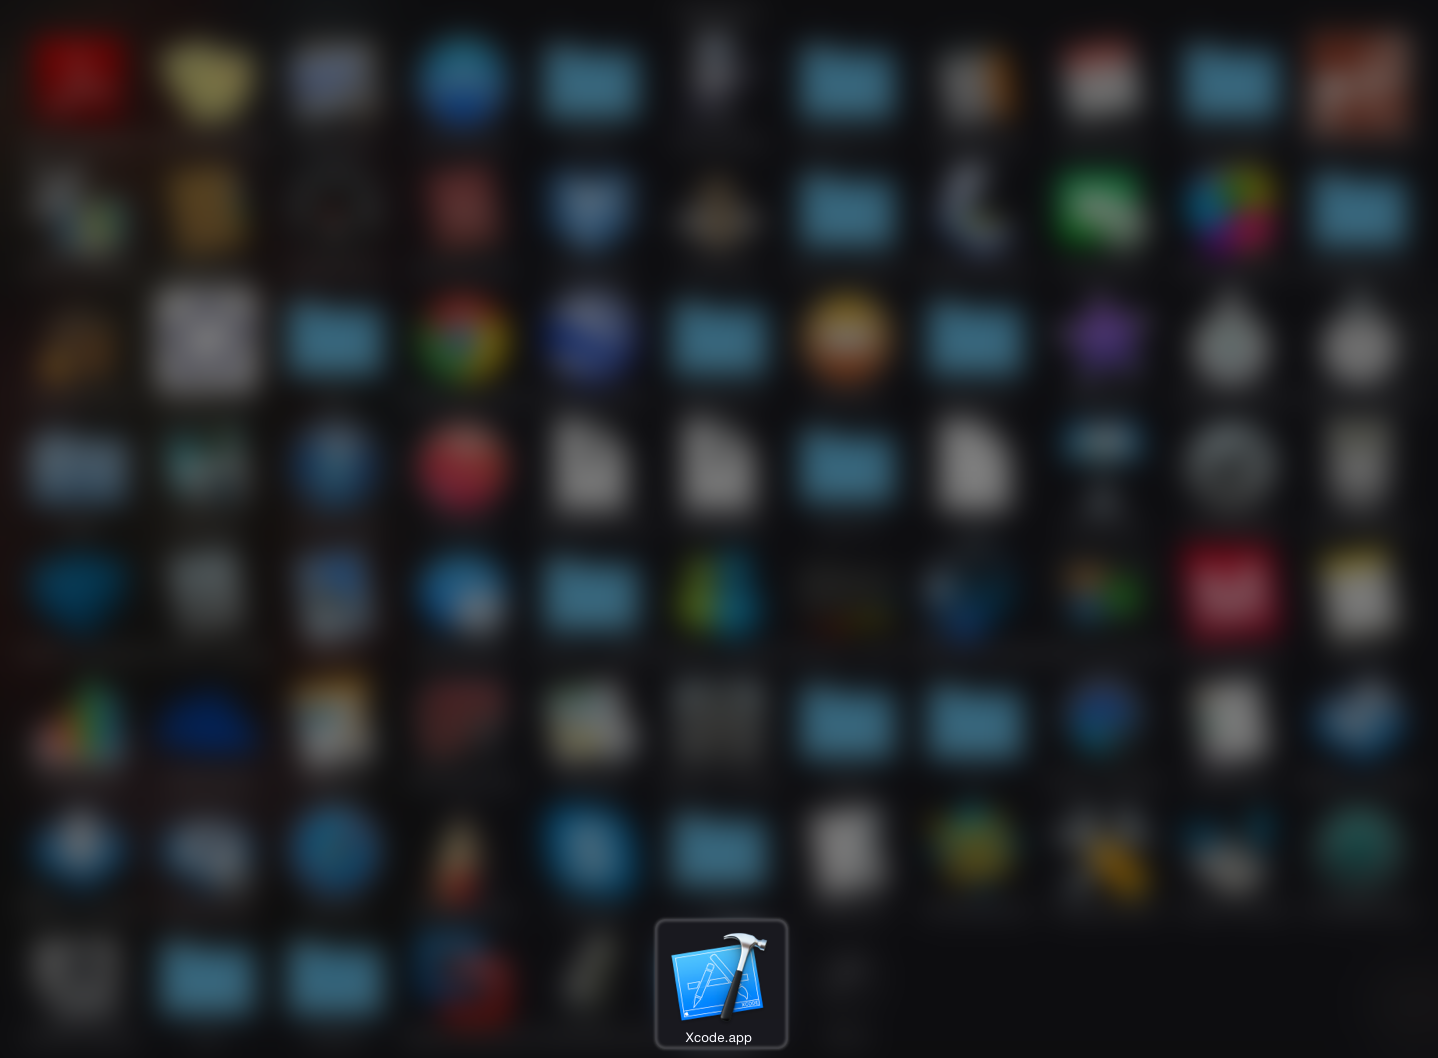
\includegraphics[scale=0.25]{\TSwiftRoot/P1-LesBasesImperatives/CH2-DecouvronsXcode/img/Launchpad}
\caption{L'icône de Xcode dans la pile \og Applications \fg{}}
\end{figure}

\subsection{Installation de la bêta}
Un lien vers la bêta de Xcode 7 est fourni sur \TSwiftUrl{https://developer.apple.com/swift/resources/}{ce site}{Swift Blog --- Ressources}, qui correspond au blog d'Apple concernant Swift.

A priori, Apple devrait vous demander de vous identifier avec une Apple ID de développeur. Si vous ne vous êtes jamais enregistré, sachez que l'enregistrement est gratuit.

\paragraph{Attention}
Il existe un programme payant, qui donne accès à beaucoup plus de choses (forum, possibilité de rapporter des bugs, certificats pour signer le code, distribution App Store), mais nous n'en avons pas besoin ici.


\section{Premier contact avec Swift : un playground}
Ouvrez Xcode.
Vous devez voir apparaitre cette fenêtre, à la colonne de droite près.
\begin{figure}[H]
\centering
\includegraphics[width=\textwidth,keepaspectratio]{\TSwiftRoot/P1-LesBasesImperatives/CH2-DecouvronsXcode/img/XcodeWindow}
\caption{Fenêtre d'accueil de Xcode}
\end{figure}

Cliquez sur << \emph{Get started with a playground} >>,
pour créer un nouveau \og playground \fg{}.
Choisissez comme plate-forme OS X, et donnez lui un nom sensé.
Une fois le projet enregistré, vous voyez apparaître une fenêtre en deux parties.

À gauche, un éditeur de texte qui contient du code Swift, à droite, une colonne dans laquelle sont affichés les résultats de chaque instruction. Cette dernière est ce qui fait la puissance d’un \emph{playground} !

\begin{figure}[H]
\centering
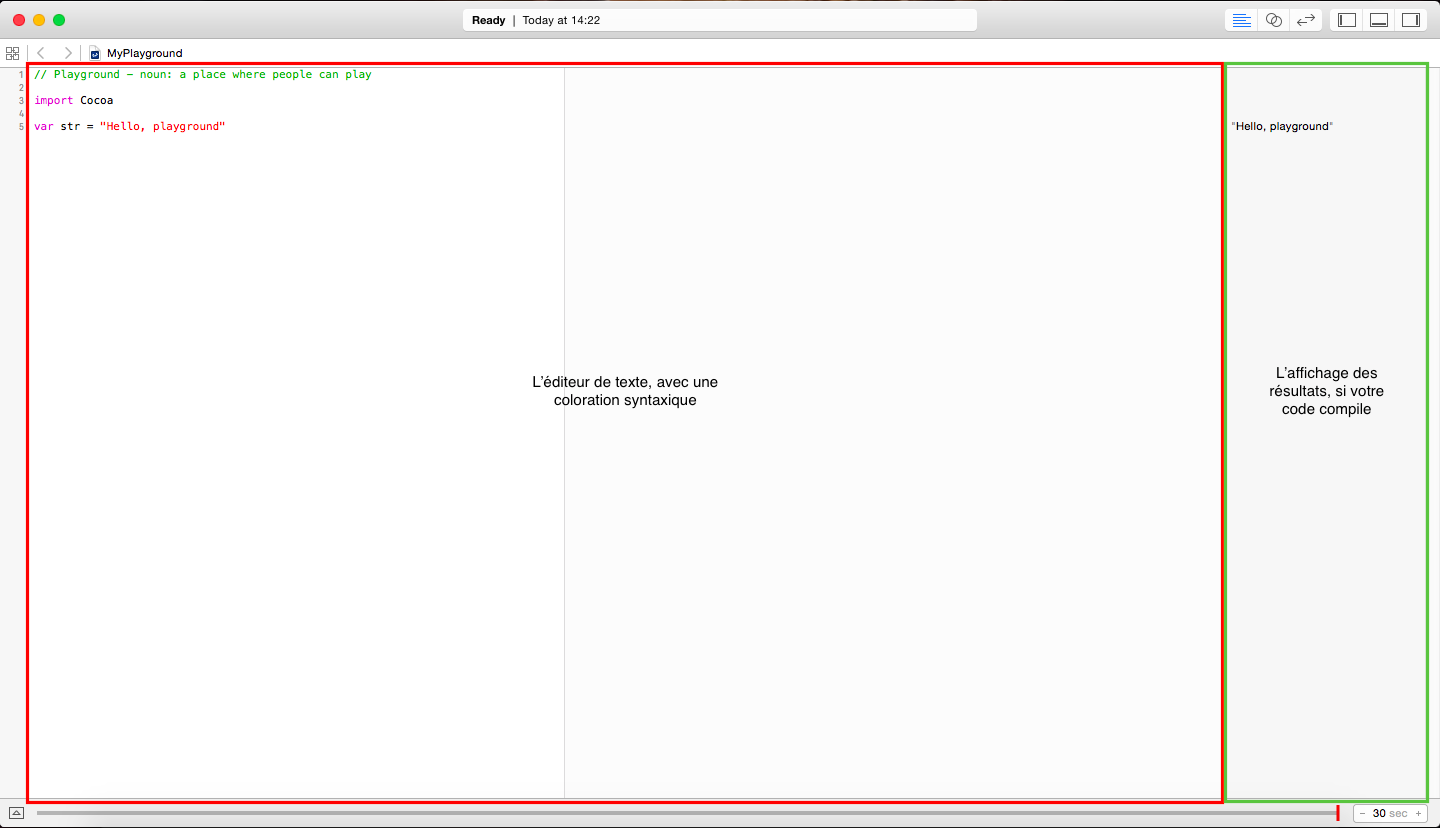
\includegraphics[width=\textwidth,keepaspectratio]{\TSwiftRoot/P1-LesBasesImperatives/CH2-DecouvronsXcode/img/Playground}
\caption{La fenêtre qui doit s’afficher lorsque vous lancez un nouveau \emph{playground}}
\end{figure}


En Swift une instruction se termine par un retour à la ligne, ou un point virgule
(si on tient absolument à mettre plusieurs instructions sur une ligne).
Vous avez normalement le code suivant,
affichant \verb"Hello, playground" en face de la troisième ligne :
\begin{listing}[H]
\caption{Code par défaut d'un \og playground \fg{} Swift}
\begin{minted}[linenos=true]{swift}
// Playground - noun: a place where people can play

import Cocoa

var str = "Hello, playground"
\end{minted}
\end{listing}

Remplacez le par le code suivant :
\begin{listing}[H]
\caption{Programme affichant \og Hello, playground \fg{}}
\begin{minted}[linenos=true]{swift}
// Playground - noun: a place where people can play

print("Hello, playground")
\end{minted}
\end{listing}

Ce code semble avoir le même effet que le précédent,
mais cela n'est vrai que dans un \emph{playground},
qui reste un environnement très particulier.

Il s’agit du premier programme que l’on montre,
par convention, dans un nouveau langage :
« \emph{Hello, World!} », qui affiche à l’écran le texte en question.

La première ligne de code est un commentaire
(ignoré royalement par le compilateur),
notion que nous étudierons dans la prochaine section ;
la deuxième, la ligne qui affiche le texte << Hello, playground ! >>
(sans les guillemets) à l’écran.
On reviendra plus en détail sur cette ligne plus tard,
mais je tenais à vous présenter ce programme,
qui est plutôt court dans ce langage
(une ligne en Swift, contre quatre lignes en C).

Vous pouvez remplacer le texte entre guillemets par le texte que vous voulez,
par exemple << \verb"Bonjour, <votre prénom> !" >>.

\mintinline{swift}{print} est la fonction
qui est chargée d’afficher à l’écran une ligne de texte.

Cette ligne de code correspond à une \emph{instruction}.

Un \emph{playground} est un outil très puissant de Xcode
puisqu’il permet de voir immédiatement
les conséquences d’une modification du code.
\section{Les Commentaires}
Un commentaire permet à l’auteur du code d’expliquer ce qu’il fait,
ou plus généralement d’introduire dans le code source
du texte ignoré par le compilateur.

Vous allez me dire, que vous ne voyez pas à quoi cela sert.
En fait, lire le code d’un autre programmeur n’est pas toujours évident,
(\og \emph{à quoi ça sert ça !? Et qu’est ce que tu veux faire là ?} \fg{}).
Pour aider les autres, ainsi que soi-même,
lorsque l'on se replonge dans son code des mois après,
il est donc indispensable d’expliquer son code.

Il est en général recommandé d'expliquer surtout
le pourquoi de certaines décisions pas forcément évidentes,
et, éventuellement, d'expliquer des algorithmes qui ne serait pas évidents.
Je vous encourage à commenter votre code de façon intensive,
car il vaut mieux trop de commentaires que pas assez.

\paragraph{Attention :}
Certains codes de cet ouvrage présente un abus dans l'usage des commentaires,
comme l'exemple expliquant les commentaires ci-après,
je vous demande de ne pas imiter ces exemples,
car il rendrait un vrai code illisible !

Il existe deux sortes de commentaires,
des commentaires qui s'arrêtent à la fin d'une ligne,
et des commentaires, éventuellement multi-lignes,
qui font ignorer au compilateur tout ce qui est contenu entre deux marqueurs.

%TODO : Refactor ?
Comme un court exemple vaut mieux qu’un long discours,
je vous laisse consulter le code suivant.

\paragraph{Attention :} À ceux qui connaissent les commentaires du C,
en Swift, les commentaires multi-lignes s'imbriquent les un dans les autres.

\begin{listing}[H]
\caption{Que de commentaires !}
\begin{minted}[linenos=true]{swift}
// Ceci est un commentaire s'arrêtant en fin de ligne.
// Cette sorte de commentaire commence par deux slash (/)
// Et s'arrête à la fin de la ligne.
print("Ceci est bien affiché")
/* Ceci est un commentaire qui s'arrête au symbole de fin */
print("Ceci est (aussi) bien affiché")
/*
Il peut s'étendre sur plusieurs lignes,
il est délimité par un symbole de début, un slash (/) suivi d'une étoile *,
et un délimiteur de fin, le même, mais à l'envers.
En swift les commentaires s'imbriquent les un dans les autres.
/*Je suis un commentaire imbriqué*/
print("Hello, playground")
Mais rien ne se passe ! On est dans un commentaire.
Fin du commentaire sur plusieurs lignes:*/
// On peut placer un commentaire après une instruction
print("Hello, playground !") // Comme ici.
// Ou même au milieu, si c'est un commentaire avec un délimiteur de fin.
print(/*Texte ici*/"Bonjour, bac à sable") // Parce qu'en Français c'est mieux.
\end{minted}
\end{listing}
Remarquez que Xcode colore les commentaires d'une couleur particulière (chez moi, le vert).

\section{Complément : Un quasi-interpréteur : La REPL Swift}
Un \emph{playground}, est un outil très puissant
puisqu’il compile et exécute immédiatement
chacune de vos instructions.

En arrière plan, Xcode compile automatiquement votre programme,
et utilise le debugger pour obtenir l’état du programme après chaque instruction.

Il existe une autre façon de jouer avec Swift,
un peu moins jolie mais encore plus rapide qu’un playground
qui reste un fichier :
La << Read Eval Print Loop >>, boucle de lecture évaluation écriture,
basé elle aussi sur le débogueur.
Si vous avez déjà utilisé la ligne de commande
ou utilisé un langage interprété comme Python,
je vous la présente ici, sinon vous pouvez sauter cette partie,
ou vous référer au tutoriel OSX \TSwiftUrl{http://openclassrooms.com/courses/domptez-votre-mac-avec-os-x-yosemite/le-terminal-dans-os-x-1}{ici}{Tutoriel sur OS X comportant un chapitre sur le Terminal},
ou à tout autre tutoriel sur la ligne de commande Unix sur Mac.

Ouvrez un Terminal Unix, et tapez \verb"swift".
Tapez ensuite une ligne de code et appuyez sur entrée.
swift affiche alors le résultat.
Pour quitter tapez \verb":quit".
En arrière plan Swift compile la ligne de code
puis l'exécute et affiche le résultat.
Attention, contrairement à un interpréteur qui lit la ligne dans son langage
et exécute les instructions correspondante,
il y a bien ici création du code binaire correspondant.
Cet outil peut être très puissant,
mais je ne le détaillerai pas ici, libre à vous de l’explorer.
\begin{listing}[H]
\caption{Exemple de sortie après un usage de la REPL Swift}
\begin{verbatim}
$ swift
Welcome to Swift!  Type :help for assistance.
  1> print("Hello, REPL")
Hello, REPL
  2> :quit
$
\end{verbatim}
% Vérifier tout ça.
\end{listing}
Par ce biais il est possible d'écrire des scripts, comme en python.



\section*{Conclusion}
\phantomsection
\addcontentsline{toc}{section}{Conclusion}
Dans cette partie vous avez :
\begin{itemize}
\item installé l'EDI\footnote{\emph{EDI} : Environnement de Développement Intégré} d'Apple ;
\item créé un nouveau \emph{playground} ;
\item appris comment afficher du texte sur la sortie standard ;
\item ce qu'est un commentaire ;
\end{itemize}
\section*{Exercice}
\phantomsection
\addcontentsline{toc}{section}{Exercice}
Passez à la pratique et faites en sorte que le \emph{playground} affiche
votre prénom dans la colonne de droite.
